\documentclass[11pt,a4paper]{article}

\usepackage[utf8]{inputenc}
\usepackage[T1]{fontenc}
\usepackage{lmodern}
\usepackage[margin=0.72in]{geometry}
\usepackage[table]{xcolor}
\usepackage{array}
\usepackage{tabularx}
\usepackage{booktabs}
\usepackage{enumitem}
\usepackage{titlesec}
\usepackage{fancyhdr}
\usepackage{lastpage}
\usepackage{hyperref}
\usepackage{tikz}

\definecolor{TextInk}{HTML}{233142}
\definecolor{HeadingBlue}{HTML}{1D3557}
\definecolor{AccentTeal}{HTML}{2A7F92}
\definecolor{AccentGold}{HTML}{C58B4E}
\definecolor{RuleGray}{HTML}{D6E0E5}
\definecolor{TableStripe}{HTML}{F3F8FA}
\definecolor{SoftTint}{HTML}{F7F4EE}
\definecolor{SoftBlue}{HTML}{EEF6F8}
\definecolor{SoftGreen}{HTML}{EEF7F0}
\definecolor{SoftRed}{HTML}{FBF0EF}

\hypersetup{
  colorlinks=true,
  linkcolor=HeadingBlue,
  urlcolor=AccentTeal,
  pdftitle={IB Geography SL Paper 2 Full Simulation - 2026-05-03},
  pdfauthor={IB Geography SL Preparation}
}

\color{TextInk}
\setlength{\parskip}{0.45em}
\setlength{\parindent}{0pt}
\setlength{\tabcolsep}{5pt}
\renewcommand{\arraystretch}{1.16}
\setlist[enumerate]{leftmargin=1.5em,itemsep=5pt,topsep=5pt}
\setlist[itemize]{leftmargin=1.35em,itemsep=3pt,topsep=4pt}

\newcolumntype{Y}{>{\raggedright\arraybackslash}X}
\newcolumntype{L}[1]{>{\raggedright\arraybackslash}p{#1}}
\newcolumntype{C}[1]{>{\centering\arraybackslash}p{#1}}

\titleformat{\section}
  {\normalfont\huge\sffamily\bfseries\color{HeadingBlue}}
  {}{0pt}{}
  [\vspace{0.12em}{\color{AccentGold}\titlerule[1pt]}]

\titleformat{\subsection}
  {\normalfont\Large\sffamily\bfseries\color{AccentTeal}}
  {}{0pt}{}

\titleformat{\subsubsection}
  {\normalfont\large\sffamily\bfseries\color{HeadingBlue}}
  {}{0pt}{}

\titlespacing*{\section}{0pt}{1.05em}{0.45em}
\titlespacing*{\subsection}{0pt}{0.78em}{0.22em}
\titlespacing*{\subsubsection}{0pt}{0.55em}{0.18em}

\pagestyle{fancy}
\setlength{\headheight}{14pt}
\fancyhf{}
\fancyhead[L]{\sffamily\color{AccentTeal}Sun 2026-05-03}
\fancyhead[R]{\sffamily\color{HeadingBlue}Paper 2 Simulation}
\fancyfoot[C]{\sffamily\color{HeadingBlue}\thepage\ of \pageref{LastPage}}
\renewcommand{\headrulewidth}{0.4pt}
\renewcommand{\footrulewidth}{0pt}

\newcommand{\term}[1]{\textcolor{HeadingBlue}{\textbf{#1}}}
\newcommand{\exam}[1]{\textcolor{AccentTeal}{\textbf{#1}}}
\newcommand{\markpts}[1]{\hfill\textbf{[#1]}}
\newcommand{\boxnote}[3]{%
\noindent\colorbox{#1}{%
  \begin{minipage}{0.965\textwidth}
  \sffamily
  \textbf{\textcolor{HeadingBlue}{#2}} #3
  \end{minipage}
}}

\begin{document}

\begin{center}
  {\sffamily\bfseries\color{HeadingBlue}\LARGE IB Geography SL}\\[0.2em]
  {\sffamily\bfseries\color{AccentTeal}\Large Paper 2 Full Simulation}\\[0.3em]
  {\sffamily\color{TextInk}Sunday 2026-05-03: Geographic Perspectives -- Global Change}
\end{center}

\vspace{0.3em}

\boxnote{SoftRed}{Practice-paper notice.}{This is an IB-style practice paper
created for revision. It is not an official IB past paper or official IB mark
scheme. Use it only under timed conditions after putting notes away.}

\section{Instructions}

\begin{tabularx}{\textwidth}{L{0.24\textwidth}Y}
\toprule
\textbf{Total time} & \term{1 hour 15 minutes}. Use the final
\term{15 minutes after the paper} for marking-guide review and an error log. \\
\textbf{Total marks} & \term{50 marks}. Section A = \term{30 marks};
Section B = \term{10 marks}; Section C = \term{10 marks}. \\
\textbf{Materials} & Question paper, answer booklet, timer, and pen. Do not
use notes during the 75-minute simulation. \\
\textbf{Structure} & Answer all three Section A structured questions, the
Section B visual stimulus task, and \term{one} Section C extended answer from
a choice of two. \\
\textbf{Review} & Open the marking guide only after the timer ends. Score
strictly and write the error log before doing any correction. \\
\bottomrule
\end{tabularx}

\subsection{Timing Checkpoints}

\rowcolors{2}{TableStripe}{white}
\begin{tabularx}{\textwidth}{L{0.18\textwidth}Y L{0.18\textwidth}}
\toprule
\textbf{Minute} & \textbf{Action} & \textbf{Marks done} \\
\midrule
0--3 & Read the instructions, source headings, and command terms. & 0 \\
3--33 & Answer Section A: Population, Climate, and Resources. & 30 \\
33--48 & Answer Section B visual stimulus task. & 40 \\
48--73 & Choose and write one Section C extended answer. & 50 \\
73--75 & Check numbering, choice, and unfinished short answers. & 50 \\
\bottomrule
\end{tabularx}
\rowcolors{2}{}{}

\newpage

\section{Section A: Core Structured Questions}

\subsection{Question 1: Population Distribution -- Changing Population}

Source A shows selected population indicators for three countries. The data are
illustrative and are provided for interpretation practice.

\rowcolors{2}{TableStripe}{white}
\begin{tabularx}{\textwidth}{L{0.24\textwidth}C{0.105\textwidth}C{0.105\textwidth}C{0.105\textwidth}C{0.105\textwidth}C{0.105\textwidth}}
\toprule
\textbf{Indicator} & \textbf{Country Alpha} & \textbf{Country Beta} &
\textbf{Country Gamma} & \textbf{Country Delta} & \textbf{Country Epsilon} \\
\midrule
Total fertility rate & 4.6 & 1.3 & 2.1 & 2.8 & 1.7 \\
Median age & 18 & 48 & 32 & 27 & 41 \\
Annual population growth & 2.7\% & -0.3\% & 0.9\% & 1.8\% & 0.2\% \\
Net migration rate & -1.2\% & 0.4\% & 0.8\% & -0.4\% & 0.2\% \\
Population aged under 15 & 43\% & 12\% & 24\% & 32\% & 16\% \\
Population aged 65 and over & 3\% & 29\% & 12\% & 6\% & 22\% \\
Urban population & 42\% & 92\% & 68\% & 55\% & 81\% \\
\bottomrule
\end{tabularx}
\rowcolors{2}{}{}

\begin{enumerate}[label=\textbf{1(\alph*)}]
  \item \exam{State} the country in Source A with the oldest population
  structure. \markpts{1}

  \item Using Source A, \exam{describe} two contrasts between Country Alpha and
  Country Beta. \markpts{4}

  \item \exam{Explain} two possible consequences of either a youthful or an
  ageing population structure. \markpts{4}

  \item \exam{Suggest} one reason why Country Gamma's population may continue
  growing even though its fertility rate is close to replacement level.
  \markpts{1}
\end{enumerate}

\subsection{Question 2: Global Climate -- Vulnerability And Resilience}

Source B compares climate-risk contexts in three places. The data are
illustrative and are provided for interpretation practice.

\rowcolors{2}{TableStripe}{white}
\begin{tabularx}{\textwidth}{L{0.2\textwidth}Y C{0.14\textwidth}C{0.18\textwidth}Y}
\toprule
\textbf{Place} & \textbf{Main climate hazards} & \textbf{Population in high-risk zone} &
\textbf{Adaptive capacity} & \textbf{Likely impacts} \\
\midrule
Low-lying delta coast & River flooding, storm surge, sea-level rise, saline
intrusion & 42\% & Low to medium & Displacement, crop loss, water
contamination, disease risk \\
High-income coastal city & Sea-level rise, coastal flooding, heatwaves & 18\%
& High & Expensive infrastructure damage, heat stress, transport disruption \\
Semi-arid rural region & Drought, heatwaves, rainfall variability & 35\% &
Low & Crop failure, livestock loss, water conflict, out-migration pressure \\
\bottomrule
\end{tabularx}
\rowcolors{2}{}{}

\begin{enumerate}[label=\textbf{2(\alph*)}]
  \item \exam{State} two climate hazards shown in Source B. \markpts{2}

  \item Using Source B, \exam{describe} two differences in vulnerability or
  resilience between the low-lying delta coast and the high-income coastal
  city. \markpts{4}

  \item \exam{Explain} two reasons why climate risk is not determined by
  physical hazard alone. \markpts{4}
\end{enumerate}

\subsection{Question 3: Global Resource Consumption And Security}

Source C compares resource consumption and resource security in three economic
contexts. The indexes are illustrative. A higher index means a higher level of
the indicator.

\rowcolors{2}{TableStripe}{white}
\begin{tabularx}{\textwidth}{L{0.28\textwidth}C{0.16\textwidth}C{0.16\textwidth}C{0.16\textwidth}Y}
\toprule
\textbf{Context} & \textbf{Energy use index per person} &
\textbf{Material footprint index per person} & \textbf{Food waste index} &
\textbf{Main resource-security issue} \\
\midrule
High-income consumer economy & 90 & 85 & 32 & High consumption,
import dependence, and waste generation \\
Emerging industrial economy & 48 & 55 & 18 & Rapid industrial demand,
pollution, and pressure on water and energy systems \\
Low-income rural economy & 12 & 15 & 6 & Low access, biomass reliance,
price shocks, and service poverty \\
\bottomrule
\end{tabularx}
\rowcolors{2}{}{}

\begin{enumerate}[label=\textbf{3(\alph*)}]
  \item \exam{Identify} one indicator from Source C showing uneven resource
  consumption. \markpts{1}

  \item Using Source C, \exam{describe} two contrasts in resource security
  between the high-income consumer economy and the low-income rural economy.
  \markpts{4}

  \item \exam{Explain} two ways resource consumption can create environmental
  or geopolitical insecurity. \markpts{4}

  \item \exam{Suggest} one stewardship strategy that could reduce resource
  insecurity. \markpts{1}
\end{enumerate}

\newpage

\section{Section B: Visual Stimulus Task}

\subsection{Question 4: Population, Climate Risk, And Resource Demand}

Source D shows four coastal megacity regions. The figures are illustrative and
are intended for visual interpretation practice.

\rowcolors{2}{TableStripe}{white}
\begin{tabularx}{\textwidth}{L{0.14\textwidth}C{0.15\textwidth}C{0.13\textwidth}C{0.13\textwidth}C{0.14\textwidth}Y}
\toprule
\textbf{Region} & \textbf{Projected population growth, 2025--2040} &
\textbf{Climate-risk index} & \textbf{Water-stress index} &
\textbf{Informal-housing share} & \textbf{Main concern} \\
\midrule
North Delta & 38\% & 86 & 64 & 41\% & Flooding and displacement \\
Dry Coast & 29\% & 74 & 91 & 28\% & Drought and desalination dependence \\
Wealthy Bay & 8\% & 58 & 37 & 3\% & High-value coastal assets \\
Island Port & 17\% & 82 & 72 & 18\% & Storm surge and import dependence \\
\bottomrule
\end{tabularx}
\rowcolors{2}{}{}

\subsubsection{Visual Source D}

Higher bars show higher values for the selected indicator.

\begin{center}
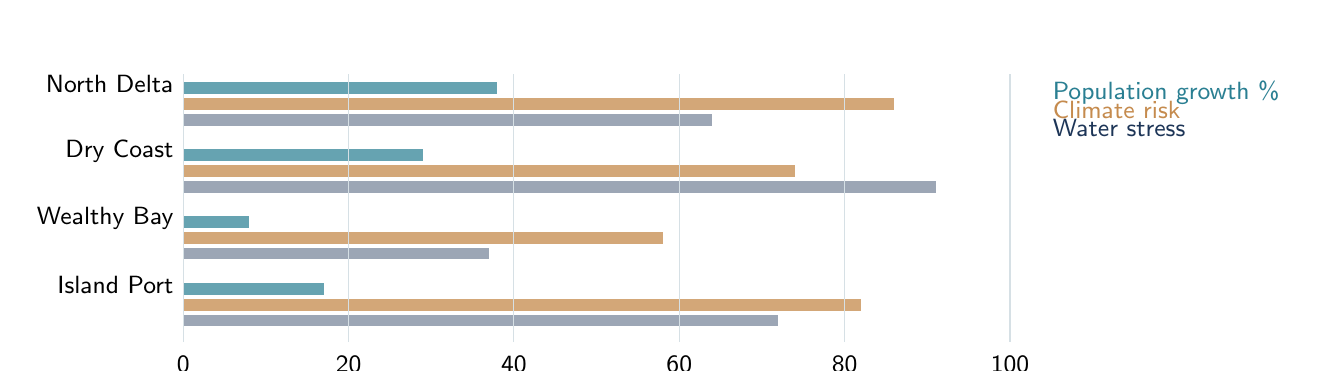
\begin{tikzpicture}[x=0.105cm,y=0.5cm, every node/.style={font=\sffamily\small}]
  \node[anchor=east] at (0,8.1) {North Delta};
  \draw[fill=AccentTeal!72, draw=none] (0,7.85) rectangle (38,8.15);
  \draw[fill=AccentGold!76, draw=none] (0,7.45) rectangle (86,7.75);
  \draw[fill=HeadingBlue!44, draw=none] (0,7.05) rectangle (64,7.35);
  \node[anchor=east] at (0,6.4) {Dry Coast};
  \draw[fill=AccentTeal!72, draw=none] (0,6.15) rectangle (29,6.45);
  \draw[fill=AccentGold!76, draw=none] (0,5.75) rectangle (74,6.05);
  \draw[fill=HeadingBlue!44, draw=none] (0,5.35) rectangle (91,5.65);
  \node[anchor=east] at (0,4.7) {Wealthy Bay};
  \draw[fill=AccentTeal!72, draw=none] (0,4.45) rectangle (8,4.75);
  \draw[fill=AccentGold!76, draw=none] (0,4.05) rectangle (58,4.35);
  \draw[fill=HeadingBlue!44, draw=none] (0,3.65) rectangle (37,3.95);
  \node[anchor=east] at (0,3.0) {Island Port};
  \draw[fill=AccentTeal!72, draw=none] (0,2.75) rectangle (17,3.05);
  \draw[fill=AccentGold!76, draw=none] (0,2.35) rectangle (82,2.65);
  \draw[fill=HeadingBlue!44, draw=none] (0,1.95) rectangle (72,2.25);
  \foreach \x in {0,20,40,60,80,100} {
    \draw[RuleGray] (\x,1.55) -- (\x,8.35);
    \node[anchor=north] at (\x,1.45) {\x};
  }
  \node[anchor=west, color=AccentTeal] at (104,7.9) {Population growth \%};
  \node[anchor=west, color=AccentGold] at (104,7.45) {Climate risk};
  \node[anchor=west, color=HeadingBlue] at (104,7.0) {Water stress};
\end{tikzpicture}
\end{center}

\begin{enumerate}[label=\textbf{4(\alph*)}]
  \item Using Source D, \exam{describe} two patterns in population growth,
  climate risk, water stress, or informal housing. \markpts{4}

  \item \exam{Suggest} two reasons why regions with similar climate-risk
  indexes may have different human impacts. \markpts{4}

  \item \exam{State} one decision-maker who could use Source D and one decision
  they might make. \markpts{2}
\end{enumerate}

\newpage

\section{Section C: Extended Answer}

Answer either Question \term{5(a)} or Question \term{5(b)}. Use named examples
where relevant. Write a clear, supported judgment.

\begin{enumerate}[label=\textbf{5(\alph*)}]
  \item Using examples, \exam{evaluate} the success of strategies to build
  resilience to climate change. \markpts{10}

  \item Using examples, \exam{to what extent} can resource stewardship reduce
  the environmental and social impacts of increasing consumption? \markpts{10}
\end{enumerate}

\vfill

\boxnote{SoftBlue}{After the timer.}{Do not look at the marking guide until
the 75-minute simulation is complete. Then use the answer booklet score sheet
and error log during the 15-minute review block.}

\end{document}
